\section{REPL commands}
\label{sec:commands}

To separate the implementation of user operations into logical units each user
operation is encapsulated within a class implementing the ``IReplCommand''
interface. See \cref{fig:uml-commands} for the design of the commands package.
After aquiring an invoker instance, the client has 2 commands available to him
by default:

\begin{itemize}
  \item :load - Implemented by LanguageCommand, loads a language from a file path.
  \item :help - Implemented by HelpCommand, prints descriptions of all available commands.
\end{itemize}

The client can define additional commands by implementing the ``IReplCommand''
interface. These commands can then be made available to the invoker by either
binding them in the default map of available commands in a guice module or by
adding the entry to the invoker at runtime using the ``addCommand'' method.

\begin{figure}[h]
  \centering
  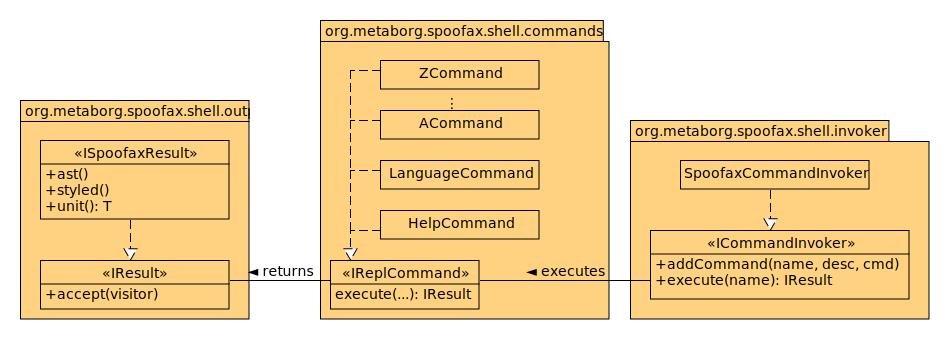
\includegraphics[width=\textwidth]{uml-commands}
  \caption{UML of the various commands clients can execute.}
  \label{fig:uml-commands}
\end{figure}
